\hypertarget{software-architecture-analysis}{%
\section{Software Architecture
Analysis}\label{software-architecture-analysis}}

\begin{tcolorbox}[colback=blue!5!white,colframe=blue!75!black]
Software architecture analysis
\begin{itemize}
    \item why evaluation of an architecture
    \item why quality attributes are important
    \item a specific method: ATAM
    \item from ATAM to fitness functions
\end{itemize}
\end{tcolorbox}

\subsection{Architecture Evaluation}
It only costs to train the people. The benefits to evaluate an Architectures are financial, early detection of problems, validation of requirement and it will certainly improve the architecture.


\hypertarget{why-evaluation-of-an-architecture}{%
\subsubsection{why evaluation of an
architecture}\label{why-evaluation-of-an-architecture}}

\begin{itemize}
\tightlist
\item
  Architecture tells about system properties

  \begin{itemize}
  \tightlist
  \item
    Effects of design decisions are predictable

    \begin{itemize}
    \tightlist
    \item
      architecture is analyzable
    \end{itemize}
  \end{itemize}
\item
  Architecture drives the software system

  \begin{itemize}
  \tightlist
  \item
    economic value
  \end{itemize}
\item
  Good evaluation methods

  \begin{itemize}
  \tightlist
  \item
    risk mitigation
  \end{itemize}

\end{itemize}


\subsubsection{when evaluation of an
architecture}
\begin{itemize}
  \item To be cost-effective: early in the lifecycle

  \subitem
    easier to correct problems
  \subitem
    quality control can be based on findings of the architectural
    evaluation

  
  
 
    \item
    Other Times in Lifecycle
    
    \subitem
    When architecture is completed but not implemented
    \subitem
    legacy system
  

\end{itemize}






\subsubsection{Techniques}
\begin{itemize}
    \item 
    Questioning techniques
    \subitem 
    Rely on though experiments which you use to create scenarios. You can also create a checklist.
    
    
    \item 
    Measureing techniques
    \subitem 
    Relies on quantitative measures of existing artifacts. You also Simulate, model and prototype and take architectural metrics to compare from.
    
    
\end{itemize}














\hypertarget{atam}{%
\subsection{ATAM}\label{atam}}

\begin{itemize}
\tightlist
\item
  ATAM = Architecture Analysis Tradeoff Method
\item
  ATAM is a comprehensive method for architecture evaluation
\item
  It shows how well an architecture satisfies particular quality goals
\item
  It provides insight into how quality goals interact (i.e., how they
  trade off)
\end{itemize}

\hypertarget{Who is involved}{%
\subsubsection{Who is involved}\label{participants}}

\begin{itemize}
\tightlist
\item
  the evaluation team

  \begin{itemize}
  \tightlist
  \item
    3 to 5 people, external to the project
  \item
    competent, unbiased, no hidden agenda
  \end{itemize}
\item
  project decision makers

  \begin{itemize}
  \tightlist
  \item
    the architect, the project manager (opt.), the customer (opt.)
  \end{itemize}
\item
  architecture stakeholders

  \begin{itemize}
  \tightlist
  \item
    developers, testers, integrators, maintainers, performance
    engineers, users, system builders, others
  \end{itemize}
\end{itemize}

\hypertarget{outcome}{%
\subsubsection{Outcome}\label{outcome}}

\begin{itemize}
\tightlist
\item
  concise documentation of the architecture
\item
  articulation of the business goals
\item
  quality requirements in terms of scenarios
\item
  mapping of architectural decisions to quality requirements
\item
  set of identified sensitivity and tradeoff points
\item
  set of risks and non-risks
\item
  prioritization of risks
\end{itemize}

\hypertarget{phases}{%
\subsubsection{Phases}\label{phases}}

\begin{itemize}
\tightlist
\item
  Phase 0: Preparation

  \begin{itemize}
  \tightlist
  \item
    project representatives brief evaluators
  \end{itemize}
\item
  Phase 1 and 2: Evaluation

  \begin{itemize}
  \tightlist
  \item
    analysis, steps given next slides
  \end{itemize}
\item
  Phase 3: Follow-up

  \begin{itemize}
  \tightlist
  \item
    evaluation team produces and delivers written evaluation report
  \end{itemize}
\end{itemize}

\hypertarget{evaluation-steps-phase-1-and-2}{%
\subsubsection{Evaluation steps (Phase 1 and
2)}\label{evaluation-steps-phase-1-and-2}}

\begin{itemize}
\tightlist
\item
  Step 1

  \begin{itemize}
  \tightlist
  \item
    present ATAM
  \end{itemize}
\item
  Step 2

  \begin{itemize}
  \tightlist
  \item
    present business drivers

    \begin{itemize}
    \tightlist
    \item
      functions
    \item
      constraints
    \item
      business goals
    \item
      architectural drivers
    \end{itemize}
  \end{itemize}
\item
  Step 3

  \begin{itemize}
  \tightlist
  \item
    present the architecture (architect) (1h!)

    \begin{itemize}
    \tightlist
    \item
      diagrams
    \end{itemize}
  \end{itemize}
\item
  Step 4

  \begin{itemize}
  \tightlist
  \item
    catalog architectural approaches

    \begin{itemize}
    \tightlist
    \item
      architectural patterns, styles, and tactics
    \end{itemize}
  \end{itemize}
\item
  Step 5

  \begin{itemize}
  \tightlist
  \item
    generate quality attribute utility table
  \end{itemize}
\item
  Step 6

  \begin{itemize}
  \tightlist
  \item
    examine the highest ranked scenarios
  \item
    evaluate architectural approaches in the light of scenarios
  \item
    identify and record candidate risks, risks, non-risks
  \end{itemize}
\item
  Step 7 (Start of Phase 2)

  \begin{itemize}
  \tightlist
  \item
    brainstorm and prioritize scenarios

    \begin{itemize}
    \tightlist
    \item
      ATAM utility table as input
    \end{itemize}
  \end{itemize}
\item
  Step 8

  \begin{itemize}
  \tightlist
  \item
    analyze architectural approach
  \end{itemize}
\item
  Step 9

  \begin{itemize}
  \tightlist
  \item
    present results
  \end{itemize}
\end{itemize}

\begin{figure}[H]
\centering
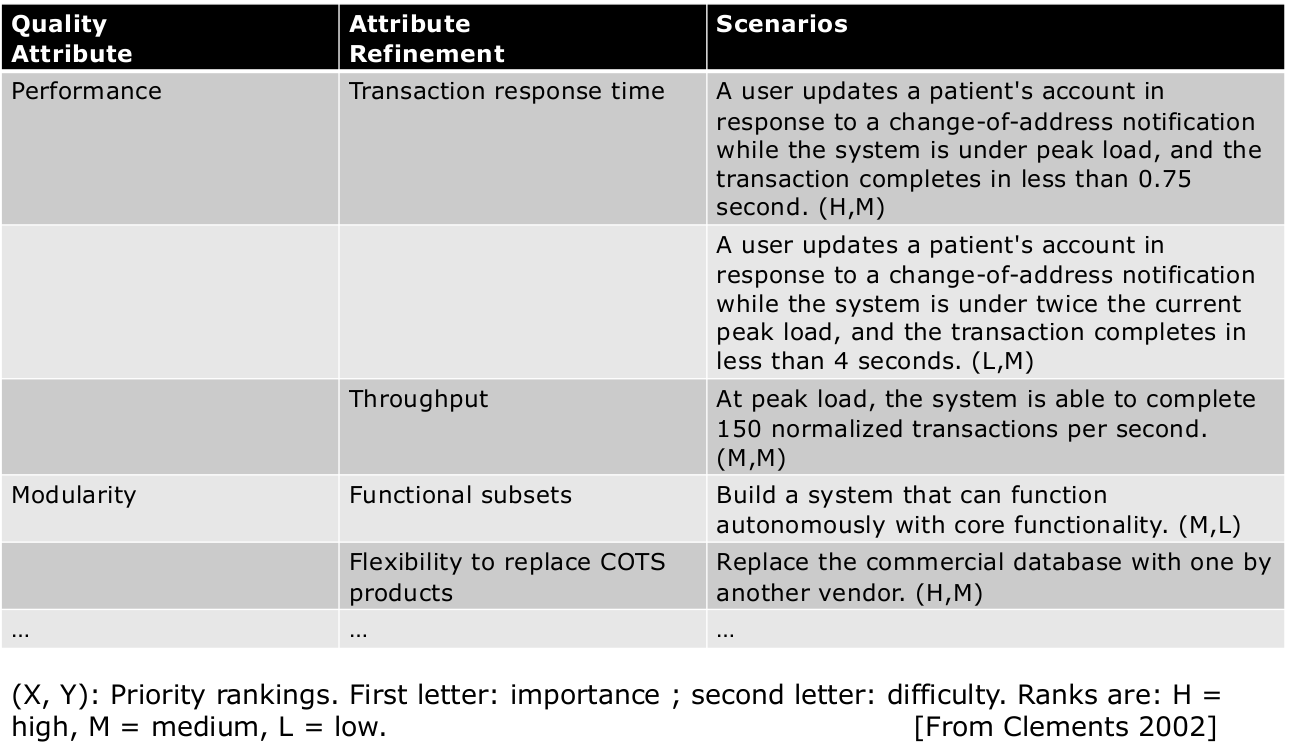
\includegraphics[width=0.5\textwidth]{figures/ATAMUtilityTable.png}
\caption{Sample Utility Table}
\end{figure}

\hypertarget{fitness-function}{%
\subsection{Fitness function}\label{fitness-function}}

Fitness functions are the unit tests for non-functional requirements.

Example Fitness Functions

\begin{itemize}
\tightlist
\item
  Static code analysis
\item
  Unit test frameworks
\item
  Penetration testing tools
\item
  Load testing tools
\item
  Monitoring tools
\item
  Logging tools
\end{itemize}


\subsection{UML Helper}
\begin{figure}[H]
\centering
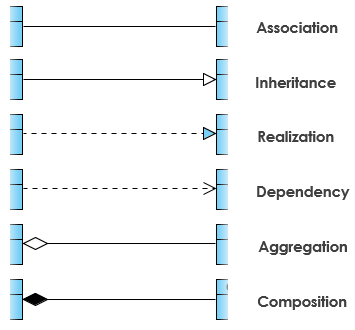
\includegraphics[width=0.5\textwidth]{figures/UMLShorties.PNG}
\caption{UML Helpers}
\end{figure}

\clearpage